\documentclass[a4paper,11pt]{article}
\usepackage{mystyle}

\begin{document}

\section{Algorithme}

\begin{enumerate}
\item
  Résoudre le problème aux valeurs propres pour trouver $(\lambda_i,\mbf{g}_i)_{i=1,\dots,M}$
\item
  Trouver les conditions aux bords $\alpha_i$ à la sortie. (sect \ref{cdtsortie})
\item
  Trouver le relévement des conditions aux bords $\mbf{a}$. (sect \ref{relev})
\item
  Ecrire Navier-Stokes pour $\mbf{v}=\mbf{a}+\mbf{u}$ où $\mbf{a}$ est connue et $\mbf{u}$ est l'inconnue.
  \begin{gather*}
    \frac{\partial \mbf{v}}{\partial t} + (\curl  \mbf{v})\times \mbf{v} + \grad q + \frac{1}{Re}\curll  \mbf{v}-\mbf{f} = 0\\
    \frac{\partial \mbf{u}}{\partial t} + (\curl \mbf{u})\times \mbf{u} + (\curl \mbf{u})\times \mbf{a} +(\curl \mbf{a})\times \mbf{u} + \grad q +\frac{1}{Re}\curll  \mbf{u} - \mbf{f_a} = 0\\
  \end{gather*}
  avec $\mbf{f_a}=\mbf{f}-\frac{\partial \mbf{a}}{\partial t} - (\curl \mbf{a})\times \mbf{a} - \curll\mbf{a}$
\item
  Injecter $\mbf{u}=\sum_{i=1}^\infty c_i(t)\mbf{g}_i(x,y,z)$ où $\mbf{g}_i$ sont connus et $c_i$ sont les inconnus.
  \begin{align*}
    \sum_{i=1}^\infty\frac{\partial c_i}{\partial t}\mbf{g}_i &+ \sum_{i=1}^\infty\sum_{j=1}^\infty c_i c_j((\curl\mbf{g}_i)\times \mbf{g}_j) + \sum_{i=1}^\infty c_i((\curl\mbf{g}_i)\times \mbf{a})\\
    & + \sum_{i=1}^\infty c_i((\curl\mbf{a})\times \mbf{g}_i) + \grad \pi_{\mbf{a}} +\frac{1}{Re}\sum_{i=1}^\infty c_i\curll\mbf{g}_i - \mbf{f_a} = 0
  \end{align*}
\item
  Formulation faible avec $\forall \varphi\in D^1 \Leftrightarrow \forall \mbf{g}_k\quad k=1,\dots,M$
  \begin{equation*}
    \frac{\partial c_k}{\partial t} + \frac{1}{Re}c_k\lambda_k^2 + \sum_{i=1}^M\sum_{j=1}^Mc_ic_jR_{ijk} + \sum_{i=1}^Mc_iR_{iak} + \sum_{i=1}^Mc_iR_{aik} = R_{fk}
  \end{equation*}
  avec :
  \begin{align*}
    R_{ijk} &= \int_\Omega((\curl\mathbf{g}_i)\times \mathbf{g}_j)\cdot\mathbf{g}_k & R_{iak} &= \int_\Omega((\curl\mathbf{g}_i)\times \mathbf{a})\cdot\mathbf{g}_k\\
    R_{aik} &= \int_\Omega((\curl\mathbf{a})\times \mathbf{g}_i)\cdot\mathbf{g}_k & R_{fk} &= \int_\Omega\mathbf{f_a}\cdot\mathbf{g}_k
  \end{align*}
\end{enumerate}

\section{Poiseuille}
On prend un écoulement de Poiseuille qui est solution de Navier-Stokes.\\
On sait aussi que l'écoulement est stationnaire donc $\frac{\partial\mbf{v}}{\partial t}=0$.\\
De plus, le terme non linéaire de Navier-Stokes est nul, il reste donc
\begin{gather}
  \frac{1}{Re}\curll\mbf{v}=-\grad p\\
  \frac{1}{Re}\left( \sum_i c_i\int_\Omega (\curll\mbf{g}_i)\cdot\mbf{g}_k + \int_\Omega (\curll\mbf{a})\cdot\mbf{g}_k \right) = \int_\Omega p\div\mbf{g}_k - \int_\Gamma p\mbf{g}_k\cdot\mbf{n}\\
  \frac{1}{Re}\lambda_k^2 c_k = -\frac{1}{Re}\int_\Omega (\curll\mbf{a})\cdot\mbf{g}_k\\
  c_k = -\frac{1}{\lambda_k^2}\int_\Omega (\curll\mbf{a})\cdot\mbf{g}_k
\end{gather}

\subsection{Relévement}
\label{relev}
Pour relever $\alpha_0$, on pourrait utiliser
\begin{equation*}
  \mbf{a}\restr{\Gamma_{1,2}}= \begin{pmatrix}
    0\\0\\\alpha_0
  \end{pmatrix}
  \quad\Longrightarrow\quad
  \curll\mbf{a}\restr{\Gamma_{1,2}}= \begin{pmatrix}
    0\\0\\-\laplace\alpha_0
  \end{pmatrix}
\end{equation*}
on rappel que $\div\mbf{a}=0$, ce qui implique que $\alpha_2=-\laplace\alpha_0$.\\
De plus, ainsi on relève $\alpha_0$ et $\alpha_2$ en même temps.\\

Cependant, il semble que lors des calculs des coefficients, les produits scalaire impliquant $\mbf{a}$ et $\mbf{g}_i$ soient nuls. Une explication peut être que la seule composante non nulle de $\mbf{a}$ est la composante normale sur les bords et que cette composante est nulle pour les $\mbf{g}_i$.\\

On utilise donc le relévement suivant :\\
On écrit $\mbf{a} = \mbf{q}_0 + \curl\bm{\psi}^1 + \bm{\psi}^2$ tel que :
\begin{align}
  \left\{
  \begin{aligned}
    \mbf{q}_i - \grad{\phi}_i &= 0 &\mbox{ sur }\Omega\\
    \div\mbf{q}_i &= 0 &\mbox{ sur }\Omega\\
    \mbf{q}_i\cdot\mbf{n} &= \alpha_i &\mbox{ sur }\Gamma
  \end{aligned}
  \right.\quad i=0,1,2\label{darcy}\\
  \nonumber\\
  \left\{
  \begin{aligned}
    \curll\bm{\psi}^i &= \mbf{q}_i &\mbox{ sur }\Omega\\
    \div\bm{\psi}^i &= 0 &\mbox{ sur }\Omega\\
    \bm{\psi}^i\cdot\mbf{n} &= 0 &\mbox{ sur }\Gamma\\
    \curl\bm{\psi}^i\cdot\mbf{n} &= 0 &\mbox{ sur }\Gamma
  \end{aligned}
  \right.\quad i=1,2\label{curlzh}
\end{align}

Où les problèmes (\ref{darcy}) sont des problèmes mixte de type Darcy que l'on peut résoudre à l'aide des éléments de Raviart-Thomas.\\
Tandis que les problèmes (\ref{curlzh}) sont des problèmes dont la solution se trouve dans l'espace $\ZZ_h$, le même que celui dans lequel nous avons résolu le problème aux valeurs propres. De plus, ce problème peut se ramener à un problème de Stokes pour lequel V. Girault donne la formulation faible suivante :
\begin{pb}
  Trouver $\bm{\psi}_i$ dans $U_0=\{\mbf{v}\in\ZZ_h\;|\; (\mbf{v},\grad q) = 0\; \forall q\in H^1\}$ tel que :
  \begin{equation*}
    \int_\Omega \curl\bm{\psi}_i\cdot\curl \mbf{v} = \int_\Omega \mbf{q}_i\cdot\mbf{v}\quad\forall\mbf{v}\in U_0
  \end{equation*}
\end{pb}

On devra donc résoudre le problème sous forme matricielle :
\begin{equation}
  C^TAC\tilde{\bm{\psi}}^i = C^T\mbf{q}_i
\end{equation}
avec :
\[ A_{ij} = \int_\Omega \curl\varphi_i\cdot\curl\varphi_j\quad\quad \bm{\psi}^i = C\tilde{\bm{\psi}}^i \]

\subsection{Résultats}
\begin{figure}[H]
  \centering
  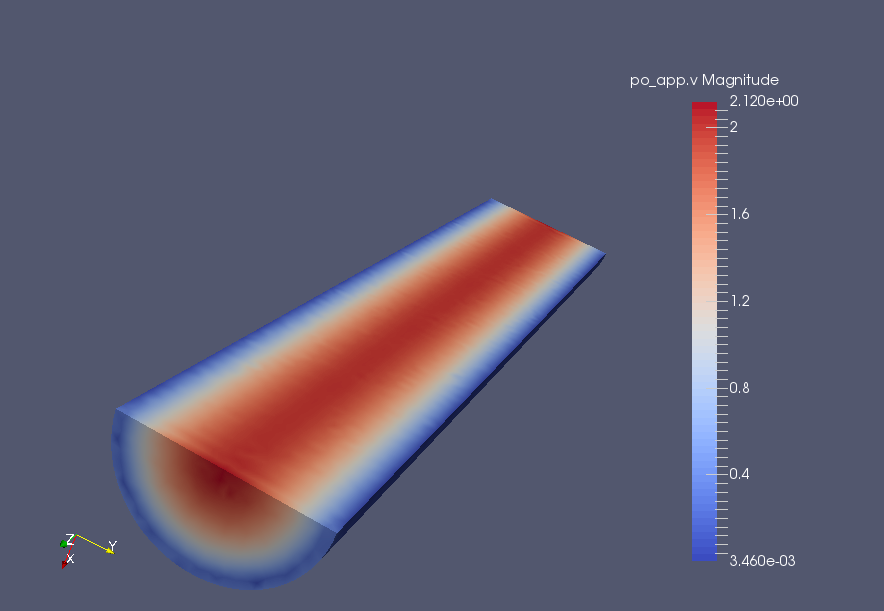
\includegraphics[scale=0.4]{vh}
  \caption{$\mbf{v}_h$ pour $h=0.08$ et $M=237$}
\end{figure}

\begin{table}[H]
  \centering
  \begin{tabular}{r|c|c||c|c}
    h & \# elts & Nh & M & $||\mbf{v}_h-\mbf{v}||_{L^2}$ \\
    \hline
    0.1 & 20434 & 26099 & 100 & 0.42 \\
    & & & 220 & 0.40 \\
    & & & 230 & 0.32 \\
    & & & 400 & 0.30 \\
    \hline
    0.08 & 36898 & 47808 & 225 & 0.36 \\
    & & & 227 & 0.27
  \end{tabular}
\end{table}

Des calculs sont encore en cours pour essayer de trouver une méthode qui fonctionne.

\section{Conditions aux bords}
\label{cdtsortie}
Sur $\Gamma_3$ :
\[ \alpha_i=0\quad i=0,1,2\quad \Longrightarrow\quad \mbf{a}=\begin{pmatrix}0\\0\\0\end{pmatrix}\quad \Longrightarrow\quad \mbf{v}=\mbf{u} \]
\begin{equation}\label{base}
  \mbox{Dans la base }
  \begin{pmatrix}
    \bm{\tau}_1\\\bm{\tau}_2\\\mbf{n}
  \end{pmatrix}
  \quad\quad \mbf{v}=
  \begin{pmatrix}
    \frac{\partial\varphi}{\partial y}\\-\frac{\partial\varphi}{\partial x}\\0
  \end{pmatrix}
\end{equation}
$\mbf{v}$ est solution de Navier-Stokes :
\[ \frac{\partial\mbf{v}}{\partial t} + (\mbf{v}\cdot\nabla)\mbf{v} + \grad p - \frac{1}{Re}\laplace\mbf{v} - \mbf{f} = 0 \]
Et donc des deux équations suivantes :
\begin{gather}
  \frac{\partial\mbf{v}_x}{\partial t} + \mbf{v}_x\frac{\partial\mbf{v}_x}{\partial x} + \mbf{v}_y\frac{\partial\mbf{v}_x}{\partial y} + \frac{\partial p}{\partial x} + \frac{1}{Re}\left(\frac{\partial^2\mbf{v}_x}{\partial x^2} + \frac{\partial^2\mbf{v}_x}{\partial y^2}\right) - \mbf{f}_x = 0 \label{NS1}\\
  \frac{\partial\mbf{v}_y}{\partial t} + \mbf{v}_x\frac{\partial\mbf{v}_y}{\partial x} + \mbf{v}_y\frac{\partial\mbf{v}_y}{\partial y} + \frac{\partial p}{\partial y} + \frac{1}{Re}\left(\frac{\partial^2\mbf{v}_y}{\partial x^2} + \frac{\partial^2\mbf{v}_y}{\partial y^2}\right) - \mbf{f}_y = 0 \label{NS2}
\end{gather}

En dérivant (\ref{NS1}) par rapport à $y$ et (\ref{NS2}) par rapport à $x$, puis en soustrayant et en utilisant (\ref{base}), on obtient :
\begin{equation}
  \frac{\partial}{\partial t}\left(\grad^2\varphi\right) + \frac{\partial\varphi}{\partial y}\frac{\partial}{\partial x}\left(\grad^2\varphi\right) - \frac{\partial\varphi}{\partial x}\frac{\partial}{\partial y}\left(\grad^2\varphi\right) = \frac{1}{Re}\nabla^4\varphi
\end{equation}

Avec des conditions aux limites à définir, on peut donc connaître $\mbf{v}=\mbf{u}$ sur $\Gamma_3$ et donc sur $\partial\Gamma_2 = \Gamma_3\cap\Gamma_2$ le bord de $\Gamma_2$.\\

De plus, en supposant les vecteurs $\bm{\tau}_1$ et $\bm{\tau}_2$ orientés comme il faut, on a :\\
Dans la base correspondant à $\Gamma_3$ :
\[
\mbf{v}\restr{\Gamma_3\cap\Gamma_2} =
\begin{pmatrix}
  \mbf{v}_1\\\mbf{v}_2\\0
\end{pmatrix}=
\begin{pmatrix}
  \frac{\partial\varphi}{\partial y}\\-\frac{\partial\varphi}{\partial x}\\0
\end{pmatrix}
\]
Dans la base correspondant à $\Gamma_2$ :
\[
\quad\mbf{v}\restr{\Gamma_2\cap\Gamma_3} =
\begin{pmatrix}
  0\\\mbf{v}_1\\\mbf{v}_2(=\alpha_0)
\end{pmatrix} =
\begin{pmatrix}
  0\\\frac{\partial\varphi}{\partial y}\\-\frac{\partial\varphi}{\partial x}
\end{pmatrix}
\]

Une idée de Benjamin pour retrouver les $\alpha_i$ à la sortie est de trouver une fonction permettant de passer de $\alpha_0\restr{\Gamma_{1,3}}$ à $\alpha_0\restr{\Gamma_{2,3}}$ et de s'en servir pour passer de $\alpha_0\restr{\Gamma_1}$ à $\alpha_0\restr{\Gamma_2}$.\\
Cette fonction reste encore à déterminer.

\end{document}
